% Created by tikzDevice version 0.12.6 on 2024-11-10 08:14:33
% !TEX encoding = UTF-8 Unicode
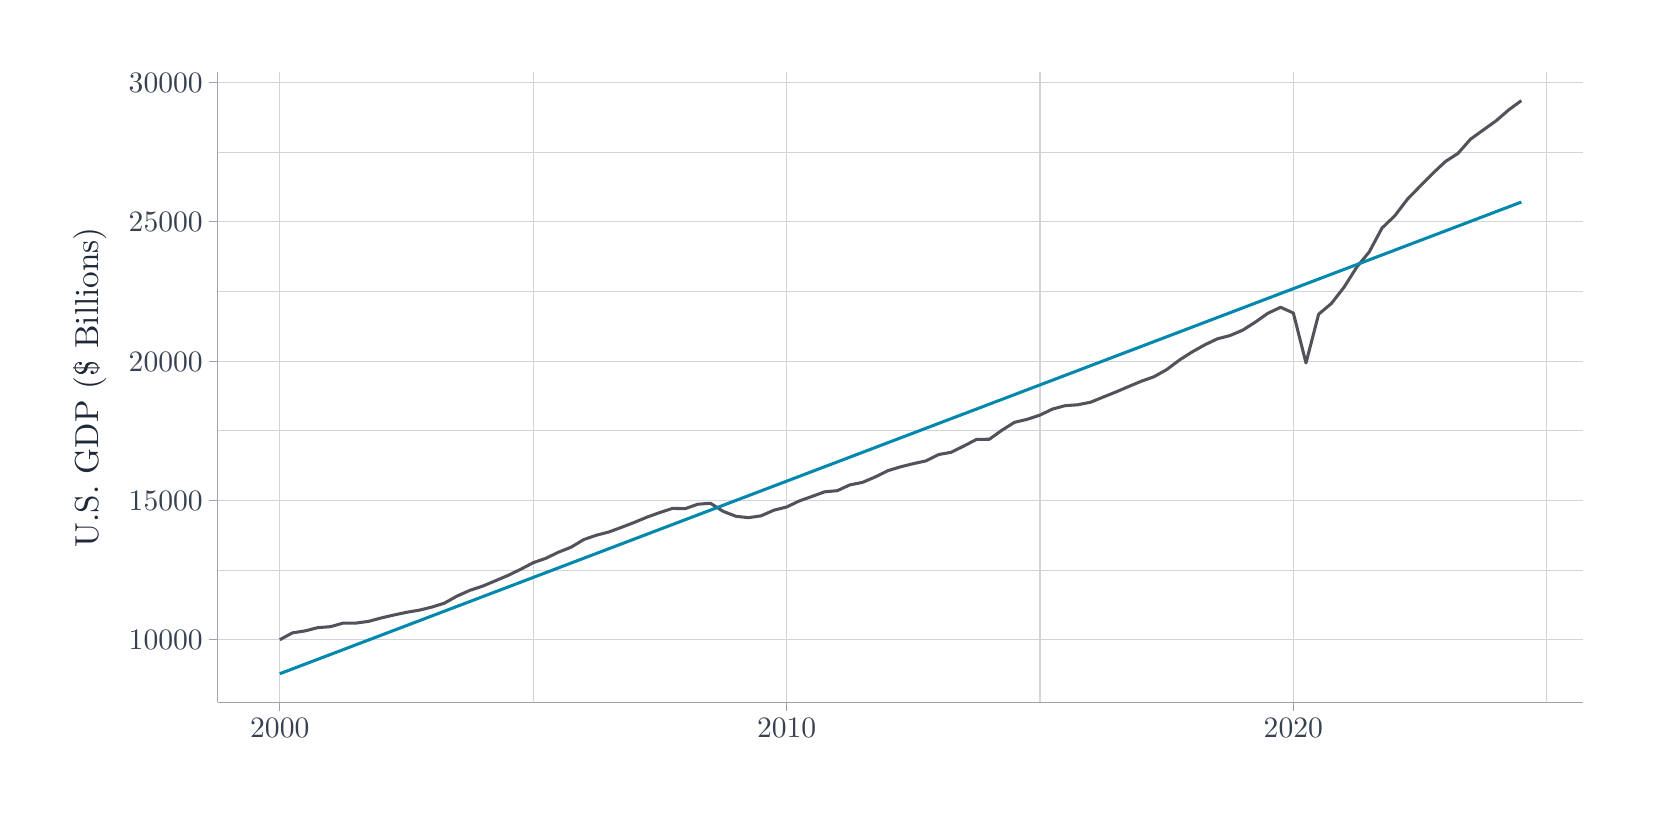
\begin{tikzpicture}[x=1pt,y=1pt]
\definecolor{fillColor}{RGB}{255,255,255}
\path[use as bounding box,fill=fillColor] (0,0) rectangle (578.16,274.63);
\begin{scope}
\path[clip] (  0.00,  0.00) rectangle (578.16,274.63);
\definecolor{drawColor}{RGB}{255,255,255}

\path[draw=drawColor,line width= 0.6pt,line join=round,line cap=round,fill=fillColor] ( -0.00,  0.00) rectangle (578.16,274.63);
\end{scope}
\begin{scope}
\path[clip] ( 68.67, 30.82) rectangle (562.16,258.63);
\definecolor{drawColor}{RGB}{255,255,255}
\definecolor{fillColor}{RGB}{255,255,255}

\path[draw=drawColor,line width= 0.6pt,line join=round,line cap=round,fill=fillColor] ( 68.67, 30.82) rectangle (562.16,258.63);
\definecolor{drawColor}{RGB}{209,213,219}

\path[draw=drawColor,line width= 0.4pt,line join=round] ( 68.67, 78.61) --
	(562.16, 78.61);

\path[draw=drawColor,line width= 0.4pt,line join=round] ( 68.67,128.96) --
	(562.16,128.96);

\path[draw=drawColor,line width= 0.4pt,line join=round] ( 68.67,179.30) --
	(562.16,179.30);

\path[draw=drawColor,line width= 0.4pt,line join=round] ( 68.67,229.64) --
	(562.16,229.64);

\path[draw=drawColor,line width= 0.4pt,line join=round] (182.67, 30.82) --
	(182.67,258.63);

\path[draw=drawColor,line width= 0.4pt,line join=round] (365.80, 30.82) --
	(365.80,258.63);

\path[draw=drawColor,line width= 0.4pt,line join=round] (548.93, 30.82) --
	(548.93,258.63);

\path[draw=drawColor,line width= 0.4pt,line join=round] ( 68.67, 53.44) --
	(562.16, 53.44);

\path[draw=drawColor,line width= 0.4pt,line join=round] ( 68.67,103.79) --
	(562.16,103.79);

\path[draw=drawColor,line width= 0.4pt,line join=round] ( 68.67,154.13) --
	(562.16,154.13);

\path[draw=drawColor,line width= 0.4pt,line join=round] ( 68.67,204.47) --
	(562.16,204.47);

\path[draw=drawColor,line width= 0.4pt,line join=round] ( 68.67,254.82) --
	(562.16,254.82);

\path[draw=drawColor,line width= 0.4pt,line join=round] ( 91.10, 30.82) --
	( 91.10,258.63);

\path[draw=drawColor,line width= 0.4pt,line join=round] (274.25, 30.82) --
	(274.25,258.63);

\path[draw=drawColor,line width= 0.4pt,line join=round] (457.35, 30.82) --
	(457.35,258.63);
\definecolor{drawColor}{RGB}{82,82,91}

\path[draw=drawColor,line width= 1.1pt,line join=round] ( 91.10, 53.46) --
	( 95.66, 55.94) --
	(100.22, 56.65) --
	(104.84, 57.83) --
	(109.45, 58.18) --
	(113.96, 59.47) --
	(118.52, 59.46) --
	(123.14, 60.09) --
	(127.75, 61.33) --
	(132.26, 62.38) --
	(136.82, 63.35) --
	(141.44, 64.13) --
	(146.05, 65.26) --
	(150.56, 66.66) --
	(155.12, 69.22) --
	(159.74, 71.29) --
	(164.35, 72.81) --
	(168.91, 74.72) --
	(173.47, 76.65) --
	(178.09, 78.89) --
	(182.70, 81.31) --
	(187.21, 82.87) --
	(191.77, 85.08) --
	(196.39, 86.91) --
	(201.00, 89.68) --
	(205.51, 91.23) --
	(210.07, 92.41) --
	(214.69, 94.12) --
	(219.30, 95.89) --
	(223.81, 97.77) --
	(228.37, 99.40) --
	(232.99,100.92) --
	(237.60,100.83) --
	(242.16,102.43) --
	(246.72,102.77) --
	(251.34, 99.84) --
	(255.95, 98.06) --
	(260.46, 97.56) --
	(265.02, 98.24) --
	(269.64,100.27) --
	(274.25,101.42) --
	(278.76,103.59) --
	(283.32,105.21) --
	(287.94,106.90) --
	(292.55,107.32) --
	(297.06,109.40) --
	(301.63,110.31) --
	(306.24,112.27) --
	(310.85,114.55) --
	(315.41,115.94) --
	(319.98,117.07) --
	(324.59,118.09) --
	(329.20,120.38) --
	(333.71,121.19) --
	(338.28,123.46) --
	(342.89,125.86) --
	(347.50,125.91) --
	(352.01,129.14) --
	(356.58,132.02) --
	(361.19,133.11) --
	(365.80,134.63) --
	(370.31,136.81) --
	(374.88,138.04) --
	(379.49,138.37) --
	(384.10,139.29) --
	(388.66,141.16) --
	(393.23,142.98) --
	(397.84,144.96) --
	(402.45,146.88) --
	(406.96,148.48) --
	(411.53,151.03) --
	(416.14,154.50) --
	(420.75,157.44) --
	(425.26,159.98) --
	(429.83,162.17) --
	(434.44,163.37) --
	(439.05,165.32) --
	(443.56,168.20) --
	(448.13,171.42) --
	(452.74,173.59) --
	(457.35,171.52) --
	(461.91,153.48) --
	(466.48,171.09) --
	(471.09,174.96) --
	(475.70,180.88) --
	(480.22,188.05) --
	(484.78,193.62) --
	(489.39,202.23) --
	(494.00,206.64) --
	(498.52,212.59) --
	(503.08,217.28) --
	(507.69,221.94) --
	(512.30,226.27) --
	(516.82,229.18) --
	(521.38,234.35) --
	(525.99,237.67) --
	(530.60,240.96) --
	(535.17,244.92) --
	(539.73,248.27);
\definecolor{drawColor}{RGB}{1,136,172}

\path[draw=drawColor,line width= 1.1pt,line join=round] ( 91.10, 41.18) --
	( 95.66, 42.91) --
	(100.22, 44.64) --
	(104.84, 46.40) --
	(109.45, 48.15) --
	(113.96, 49.86) --
	(118.52, 51.60) --
	(123.14, 53.35) --
	(127.75, 55.10) --
	(132.26, 56.82) --
	(136.82, 58.55) --
	(141.44, 60.30) --
	(146.05, 62.05) --
	(150.56, 63.77) --
	(155.12, 65.50) --
	(159.74, 67.25) --
	(164.35, 69.01) --
	(168.91, 70.74) --
	(173.47, 72.47) --
	(178.09, 74.22) --
	(182.70, 75.98) --
	(187.21, 77.69) --
	(191.77, 79.42) --
	(196.39, 81.18) --
	(201.00, 82.93) --
	(205.51, 84.64) --
	(210.07, 86.38) --
	(214.69, 88.13) --
	(219.30, 89.88) --
	(223.81, 91.60) --
	(228.37, 93.33) --
	(232.99, 95.08) --
	(237.60, 96.83) --
	(242.16, 98.57) --
	(246.72,100.30) --
	(251.34,102.05) --
	(255.95,103.81) --
	(260.46,105.52) --
	(265.02,107.25) --
	(269.64,109.01) --
	(274.25,110.76) --
	(278.76,112.47) --
	(283.32,114.21) --
	(287.94,115.96) --
	(292.55,117.71) --
	(297.06,119.42) --
	(301.63,121.16) --
	(306.24,122.91) --
	(310.85,124.66) --
	(315.41,126.40) --
	(319.98,128.13) --
	(324.59,129.88) --
	(329.20,131.63) --
	(333.71,133.35) --
	(338.28,135.08) --
	(342.89,136.83) --
	(347.50,138.59) --
	(352.01,140.30) --
	(356.58,142.03) --
	(361.19,143.79) --
	(365.80,145.54) --
	(370.31,147.25) --
	(374.88,148.99) --
	(379.49,150.74) --
	(384.10,152.49) --
	(388.66,154.22) --
	(393.23,155.96) --
	(397.84,157.71) --
	(402.45,159.46) --
	(406.96,161.18) --
	(411.53,162.91) --
	(416.14,164.66) --
	(420.75,166.41) --
	(425.26,168.13) --
	(429.83,169.86) --
	(434.44,171.61) --
	(439.05,173.37) --
	(443.56,175.08) --
	(448.13,176.81) --
	(452.74,178.57) --
	(457.35,180.32) --
	(461.91,182.05) --
	(466.48,183.79) --
	(471.09,185.54) --
	(475.70,187.29) --
	(480.22,189.00) --
	(484.78,190.74) --
	(489.39,192.49) --
	(494.00,194.24) --
	(498.52,195.96) --
	(503.08,197.69) --
	(507.69,199.44) --
	(512.30,201.19) --
	(516.82,202.91) --
	(521.38,204.64) --
	(525.99,206.39) --
	(530.60,208.15) --
	(535.17,209.88) --
	(539.73,211.61);
\end{scope}
\begin{scope}
\path[clip] (  0.00,  0.00) rectangle (578.16,274.63);
\definecolor{drawColor}{RGB}{156,163,175}

\path[draw=drawColor,line width= 0.3pt,line join=round] ( 68.67, 30.82) --
	( 68.67,258.63);
\end{scope}
\begin{scope}
\path[clip] (  0.00,  0.00) rectangle (578.16,274.63);
\definecolor{drawColor}{RGB}{55,65,81}

\node[text=drawColor,anchor=base east,inner sep=0pt, outer sep=0pt, scale=  1.07] at ( 63.27, 49.77) {10000};

\node[text=drawColor,anchor=base east,inner sep=0pt, outer sep=0pt, scale=  1.07] at ( 63.27,100.11) {15000};

\node[text=drawColor,anchor=base east,inner sep=0pt, outer sep=0pt, scale=  1.07] at ( 63.27,150.46) {20000};

\node[text=drawColor,anchor=base east,inner sep=0pt, outer sep=0pt, scale=  1.07] at ( 63.27,200.80) {25000};

\node[text=drawColor,anchor=base east,inner sep=0pt, outer sep=0pt, scale=  1.07] at ( 63.27,251.14) {30000};
\end{scope}
\begin{scope}
\path[clip] (  0.00,  0.00) rectangle (578.16,274.63);
\definecolor{drawColor}{RGB}{156,163,175}

\path[draw=drawColor,line width= 0.3pt,line join=round] ( 65.67, 53.44) --
	( 68.67, 53.44);

\path[draw=drawColor,line width= 0.3pt,line join=round] ( 65.67,103.79) --
	( 68.67,103.79);

\path[draw=drawColor,line width= 0.3pt,line join=round] ( 65.67,154.13) --
	( 68.67,154.13);

\path[draw=drawColor,line width= 0.3pt,line join=round] ( 65.67,204.47) --
	( 68.67,204.47);

\path[draw=drawColor,line width= 0.3pt,line join=round] ( 65.67,254.82) --
	( 68.67,254.82);
\end{scope}
\begin{scope}
\path[clip] (  0.00,  0.00) rectangle (578.16,274.63);
\definecolor{drawColor}{RGB}{156,163,175}

\path[draw=drawColor,line width= 0.3pt,line join=round] ( 68.67, 30.82) --
	(562.16, 30.82);
\end{scope}
\begin{scope}
\path[clip] (  0.00,  0.00) rectangle (578.16,274.63);
\definecolor{drawColor}{RGB}{156,163,175}

\path[draw=drawColor,line width= 0.3pt,line join=round] ( 91.10, 27.82) --
	( 91.10, 30.82);

\path[draw=drawColor,line width= 0.3pt,line join=round] (274.25, 27.82) --
	(274.25, 30.82);

\path[draw=drawColor,line width= 0.3pt,line join=round] (457.35, 27.82) --
	(457.35, 30.82);
\end{scope}
\begin{scope}
\path[clip] (  0.00,  0.00) rectangle (578.16,274.63);
\definecolor{drawColor}{RGB}{55,65,81}

\node[text=drawColor,anchor=base,inner sep=0pt, outer sep=0pt, scale=  1.07] at ( 91.10, 18.07) {2000};

\node[text=drawColor,anchor=base,inner sep=0pt, outer sep=0pt, scale=  1.07] at (274.25, 18.07) {2010};

\node[text=drawColor,anchor=base,inner sep=0pt, outer sep=0pt, scale=  1.07] at (457.35, 18.07) {2020};
\end{scope}
\begin{scope}
\path[clip] (  0.00,  0.00) rectangle (578.16,274.63);
\definecolor{drawColor}{RGB}{31,41,55}

\node[text=drawColor,rotate= 90.00,anchor=base,inner sep=0pt, outer sep=0pt, scale=  1.20] at ( 25.43,144.72) {U.S. GDP (\$ Billions)};
\end{scope}
\end{tikzpicture}
